\section{Memory Hierarchy}
I principi fondamentali che andremo a vedere sono legati alle tecnologie con cui vengono costruite le memorie, la gerarchia delle varie tipologie di memorie, le memorie caches ed in fine come andare a misurare e migliorare le performance delle caches.

\subsection{Memory Technologies}
Partiamo dicendo che esistono varie tipologie di memorie, che possono essere distinte in primo luogo in \textbf{memorie volatili}, e \textbf{memorie non volatili}. Fra memorie volatili abbiamo:
\begin{wrapfigure}{r}{5cm}
    \centering
    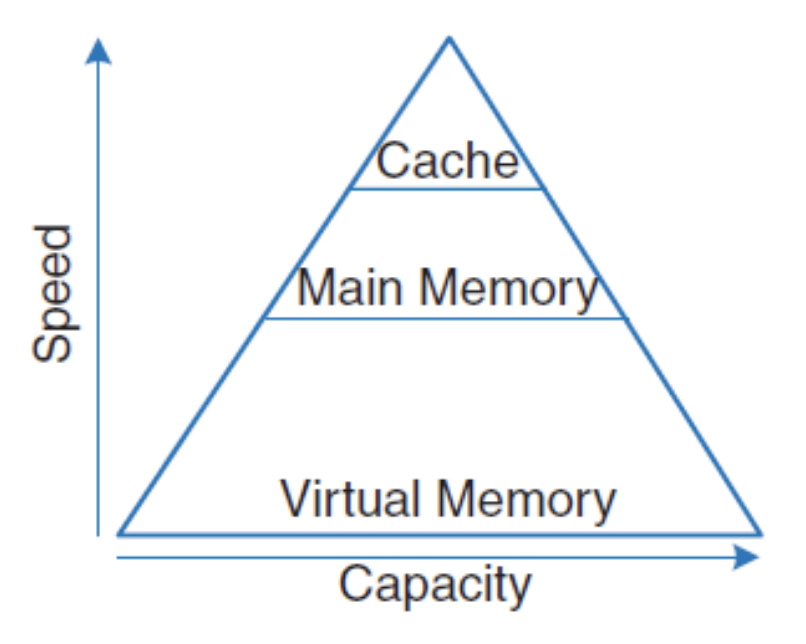
\includegraphics[width=4cm]{images/memory-hierarcgy.png}
    \caption{Gerarchia memoria}
\end{wrapfigure}

\begin{itemize}
    \item Latches, flip-flops, register files (o semplici registri).
    \item SRAM (Static Random-Access Memory).
    \item DRAM (Dynamic Random-Access Memory).
\end{itemize}

\hspace{-15pt}Fra le memorie non volatile invece ci sono:
\begin{itemize}
    \item ROM
    \item NVRAM
    \item Flash memory
    \item Magnetic disks
    \item And others ...
\end{itemize}

\subsection{Cost vs Capacity vs Access Time}
Un altro interessanto confronto da fare fra le memorie e relativo ai costi, le capacità ed il tempo di accesso per ciascuna.
\begin{itemize}
    \item \textbf{SRAM}. Access Time (ns): 0.5 - 1, Bandwidth (GB/s): 25+. Price (\$/GB): 5000. Used for registers and caches.
    \item \textbf{DRAM}. Access Time (ns): 10 - 50, Bandwidth (GB/s): 10. Price (\$/GB): 7. Used for RAM.
    \item \textbf{Flash memory}. Access Time (ns): 20.000 (20us), Bandwidth (GB/s): 0.5. Price (\$/GB): 0.40. Used for: SSD disk (secondary and virtual memory - non volatile).
    \item \textbf{Magnetic disks}: Access Time (ns): 5.000.000 (5ms), Bandwidth (GB/s): 0.75. Price (\$/GB): 0.05. Used for: HDD disk (secondary/tertiary storage - non volatile).
\end{itemize}

\hspace{-15pt}Da questa classificazione possiamo trarre alcune regole generali:
\begin{itemize}
    \item Le memorie di grandi dimensioni sono solitamente lente e economiche.
    \item Le memorie di piccole dimensioni sono più veloci ma anche più costose.
\end{itemize}

\hspace{-15pt}Da qui possiamo capire che nella selezione della memorie va trovato un compromesso fra i parametri visti precedentemente per andare ad avere memorie sufficientemente grandi per contenere i dati richiesti ma allo steso tempo sufficientemente veloci per evitare il \textbf{von Neumann Bottleneck}.

\subsection{Von Neumann architecture}
\begin{wrapfigure}{r}{6.5cm}
    \vspace{-25pt}
    \centering
    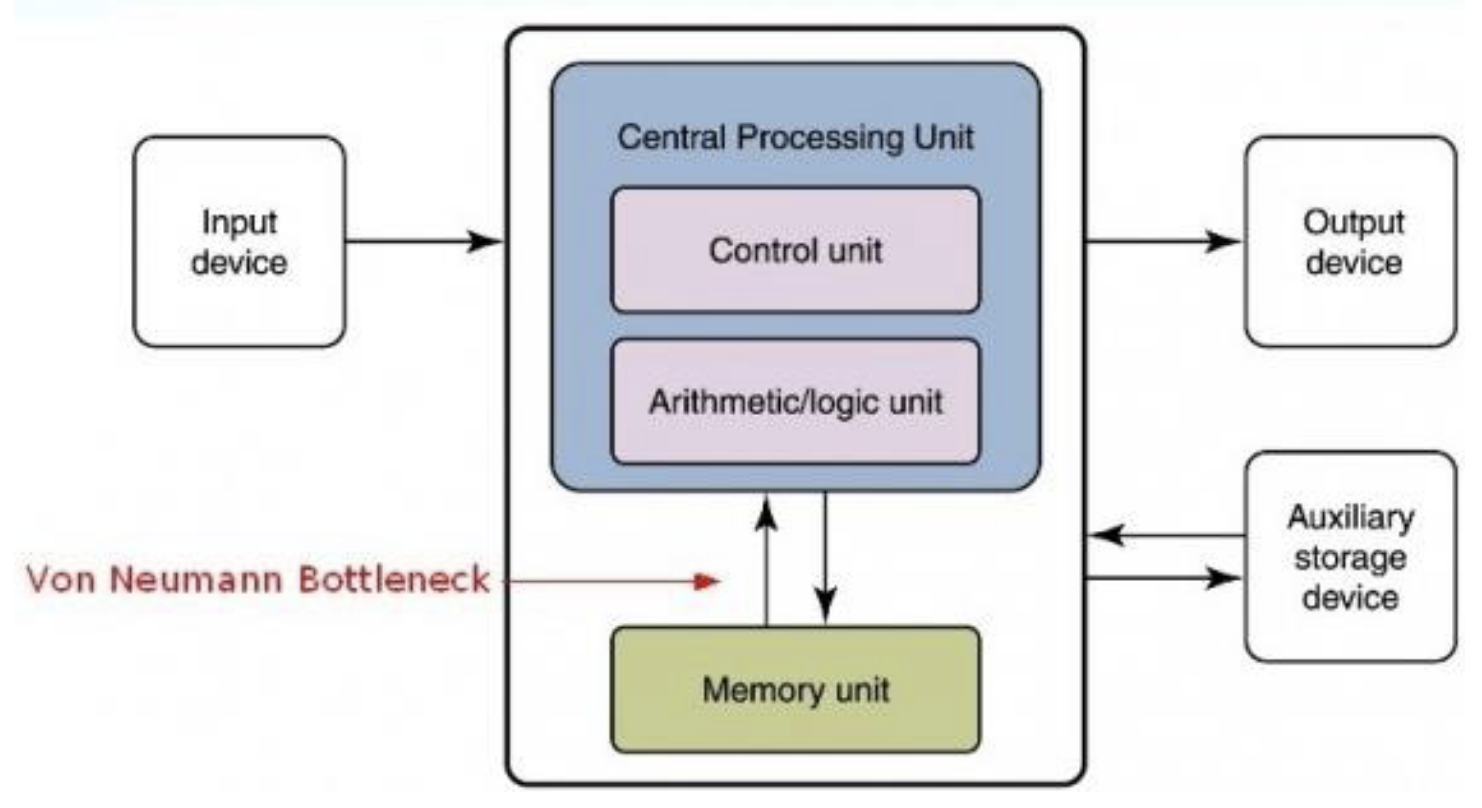
\includegraphics[width=6cm]{images/von-numan.png}
    \caption{Von-Neumann}
\end{wrapfigure}
Le perfomance dei computer sono limitate nella velocità della CPU dal trasferimento di dati fra le memorie esterne dall'unità di calcolo.\\
Per andare a mitigare questo problema andiamo a inserire memorie più piccole vicino al processore, mentre più ci si allontana si avrà memorie di grosse ma anche più lente. Da qui vorremmo che il processore lavori alla velocità della memoria più vicina.\\\\

\begin{wrapfigure}{l}{6.5cm}
    \vspace{-10pt}
    \centering
    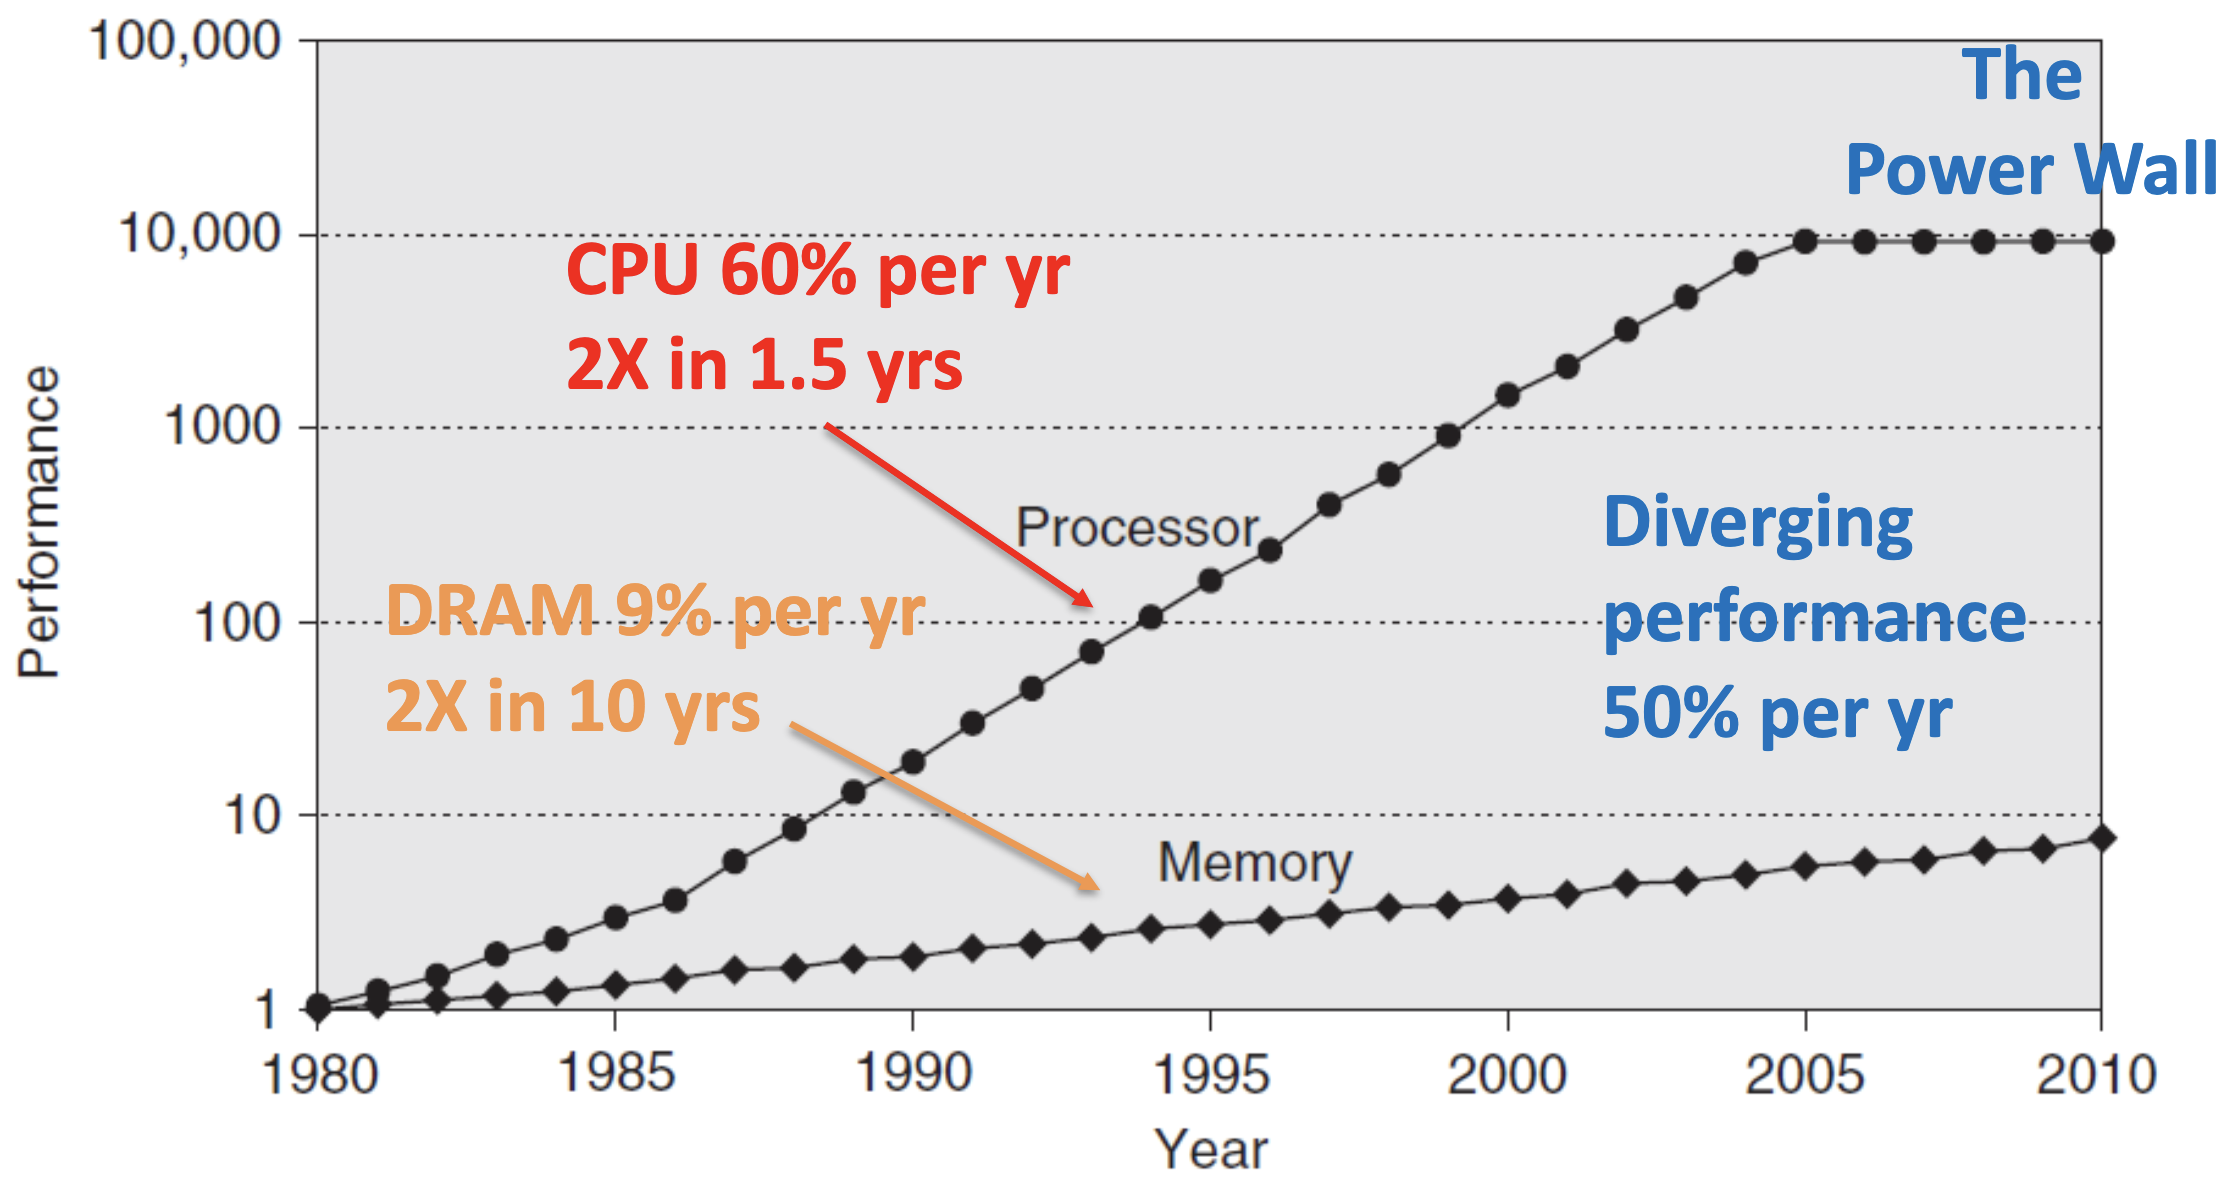
\includegraphics[width=6cm]{images/von-newmann-bottleneck.png}
    \caption{Von-Neumann Bottleneck}
\end{wrapfigure}
L'obbiettivo è quindi di fornire l'illusione di avere una memoria grande quando al memoria più lontana e veloce quando la memoria più vicina.
Per creare questa illusione andiamo a far risiedere i dati inizialmente nel livello più lontano e più capiente. Per far accedere il processore bisognerà a andare a spostare i dati. Un primo problema è che fra le memorie diverse i dati saranno salvati in indirizzi diversi, che quindi dovranno esser mappati.\\\\
Un altro aspetto è che i trasferimenti di memoria possono non essere di una singola parola, un altro problema è che se un dato viene modificato in una memoria bisogna decidere come propagare le modifiche. Capiamo dunque che si sono un insieme di problemi per andare a implementare questa soluzione.


\subsection{Terminologia}
Introduciamo innanzitutto un po' di terminologia che ci servirà successivamente.

\begin{definition}[Hit e Miss]
Se i dati richiesti dal processore compaiono in qualche blocco nel livello di memoria più vicino, si parla di hit. In caso contrario, la richiesta viene definita miss e si accede al livello di memoria successivo per recuperare il blocco contenente i dati richiesti.
\end{definition}

\begin{definition}[Hit rate]
    Il hit rate (frequenza di successi) è la frazione di accessi alla memoria rilevati nel livello superiore (ovvero, più vicino alla CPU), utilizzata come misura delle prestazioni della gerarchia.
\end{definition}

\begin{definition}[Miss rate]
    Il miss rate è la frazione di accessi alla memoria non trovati nel livello superiore.
\end{definition}

\begin{definition}[Miss penalty]
    La miss penalty è il tempo necessario per sostituire un blocco nel livello n con il blocco corrispondente dal livello n-1.
\end{definition}

\begin{definition}[Miss time]
    Il miss time è il tempo per ottenere l'elemento in caso di tempo di miss. miss time = penalità di miss + tempo di hit.
\end{definition}

Il miss rate ed il hit rate se li vogliamo calcolare lo si può fare con la seguenti formule:
\begin{equation}
    MR = \frac{\text{Number of misses}}{\text{Number of total memory access}} = 1 - HR
\end{equation}
\begin{equation}
    MR = \frac{\text{Number of hits}}{\text{Number of total memory access}} = 1 - MR
\end{equation}

Definiamo anche il AMAT (Average Memory Access Time)
\begin{equation}
    AMAT = t_{M0} + MR_{M0} * (t_{M1} + MR_{M1} * (t_{M2} + MR_{M2} * (t_{M3} + \dots)))
\end{equation}
$t_{M0}$ = hit time, $MR_{M0}$ = miss rate, $(t_{M1} + MR_{M1} * (t_{M2} + MR_{M2} * (t_{M3} + \dots))$ = miss penalty.

\begin{observation}
Se l'hit rate è abbastanza alto, la gerarchia della memoria ha un tempo di accesso effettivo vicino a quello del livello più alto (e più veloce) e una dimensione uguale a quella del livello più basso (e più grande).
\end{observation}

\subsection{The locality principle}
Il principio di località di riferimento (o locality principle) si riferisce al fenomeno nel quale un programma tende ad accedere alla stessa locazione di memoria per un determinato periodo. Possiamo osservare che, se il programma fa riferimento ad una locazione di memoria allora la stessa locazione di memoria verrà riutilizzerà a breve con alta probabilità. Inoltre, gli elementi "vicini" alla posizione di memoria appena raggiunta saranno presto referenziati con un'alta probabilità. \\

Il principio di località è la forza trainante che rende la gerarchia della memoria funzionante. Esso infatti incrementa la probabilità di riutilizzare dei blocchi di dati che erano stati precedente mossi da un livello n ad un livello n-1, questo riduce il miss rate.

\subsubsection{Locality characterization}
Andiamo a distinguere due tipologie di località. 
\begin{itemize}
    \item \textbf{La località temporale} (o riuso di dati): i dati riferiti precedentemente probabilmente li riferirò nuovamente in un breve lasso di tempo. \\\\Esempio: consideriamo il seguente codice: for(int i=0; i<10; i++) $\{$s1 += i; s2 -= 1;$\}$\\
    In questo caso le locazioni di memoria che contengono s1 ed s2 hanno località temporale.\\\\
    Dunque se all'interno della gerarchia della memoria andiamo a tenere i dati più recenti, secondo il principio di località ci riaccenderò con la CPU nuovamente a breve termine.
    \item \textbf{Località spaziale} dati vicini a quelli a cui sto riferendo saranno saranno probabilemete utilizzati a breve.
    \\\\Esempio: consideriamo il seguente codice: for(int i=0; i<10; i++) $\{$func(A[i])$\}$\\
    In questo caso le locazioni di memoria dell'array hanno località spaziale, visto che sono implementate in modo contiguo.\\\\
    Dunque se all'interno della gerarchia della memoria andiamo a tenere i dati vicini a quelli in utilizzo, secondo il principio di località ci saranno grosse probabilità di accederci con la CPU.
\end{itemize}


\subsection{Traferimiento dati}
I dati si trasferiscono solamente attraverso due memorie adiacenti. Per ottimizzare il caricamento dei dati esso viene fatto come \textbf{blocchi} di granularità di dati. La dimensione dei blocchi può cambiare attraverso i livelli. Per la cache i blocchi vengono chiamati cache line o cache block (il loro valore tipico è 64 - 128 bytes). Per le RAM invece abbiamo pagine si segmenti, mentre per i dischi abbiamo blocchi di dischi.\\

\hspace{-15pt}Consideriamo il seguente codice di C è il suo corrispettivo in assembly.
\begin{figure}[!h]
\begin{minipage}[t]{0.45\linewidth}
\centering
\begin{lstlisting}
// Sum and A are global variables
int i;
for(int i=0; sum=0; i<N, i++){
    sum += A[i];
}
// One possible compilation ====>
\end{lstlisting}
\end{minipage}
\hspace{.35cm}
\begin{minipage}[t]{0.45\linewidth}
\begin{lstlisting}
loop: cmp r3, r3
      beq end
      ldr r12, [r0, r3, lsl #2]
      ldr r4, [r1]
      add r4, r4, r12
      str r4, [r1]
      add r3, r3, #1
      b loop
end: ...
\end{lstlisting}
\end{minipage}
\end{figure}

In questo frammento di codice viene eseguito il loop N volte, e quindi ogni struttura viene richiesta N volte in maniera sequenziale, in questo caso sia la localizzazione temporale che spaziale viene utilizzata.\\
'Sum' è ripetutamente letta e scritta, quindi utilizza la località temporale, 'A' è salvata come un insieme contiguo di celle di memoria, quindi utilizzerà la località spaziale.
\newpage
\subsubsection{Cache Memories}
La cache memory è la memoria più vicina al processore, solitamente sono le SRAM, ma alcune volte sono implementate anche come DRAM. Ad oggi tutte le architetture hanno alcuni livelli di cache integrati nel chip, essa può essere più o meno grande, ne può avere più di un livello.

\subsubsection{Gestione del movimento dei dati}
Fra il primo livello di cache e i registri il trasferimento è gestione dal compilato. Il trasferimento fra caches e RAM viene invece gestito dalla microarchitettura. In fine la gestione dei trasferimenti fra RAM e storate viene fatta dal sistema operativo.

\begin{figure}[h!]
    \centering
    \begin{subfigure}{.45\textwidth}
        \centering
        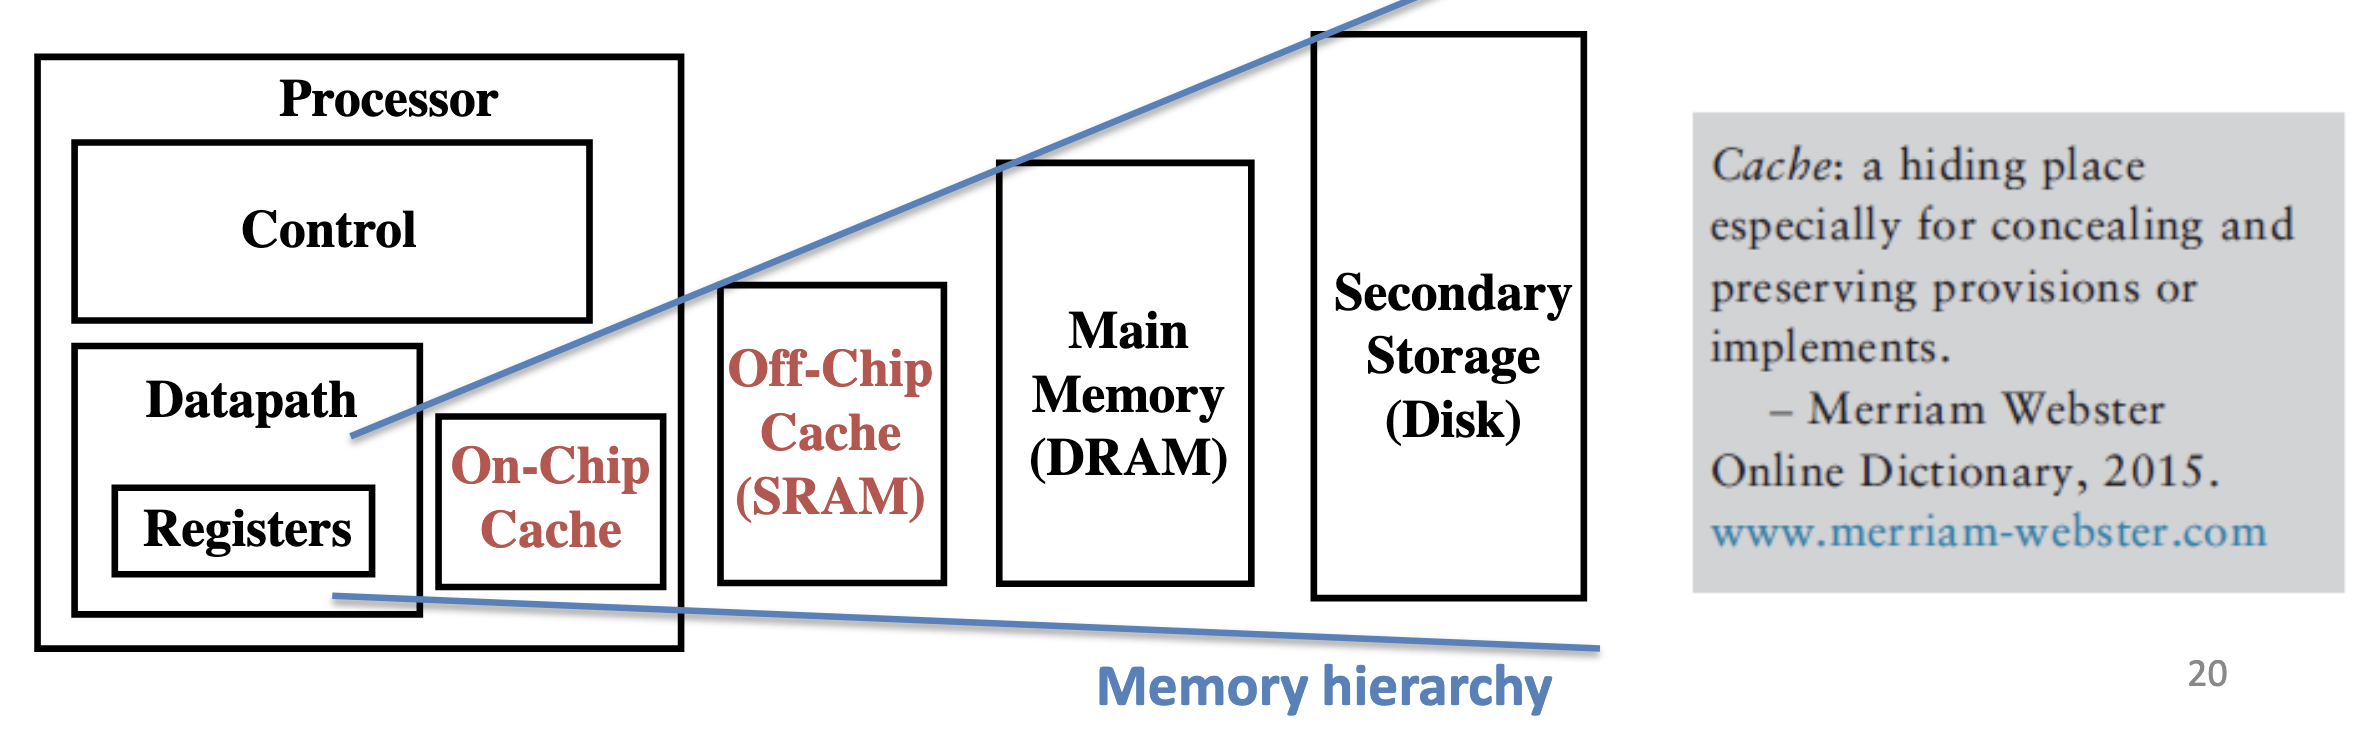
\includegraphics[width=6.5cm]{images/cache-memories.png}
        \caption{}
    \end{subfigure}
    \begin{subfigure}{.45\textwidth}
        \centering
        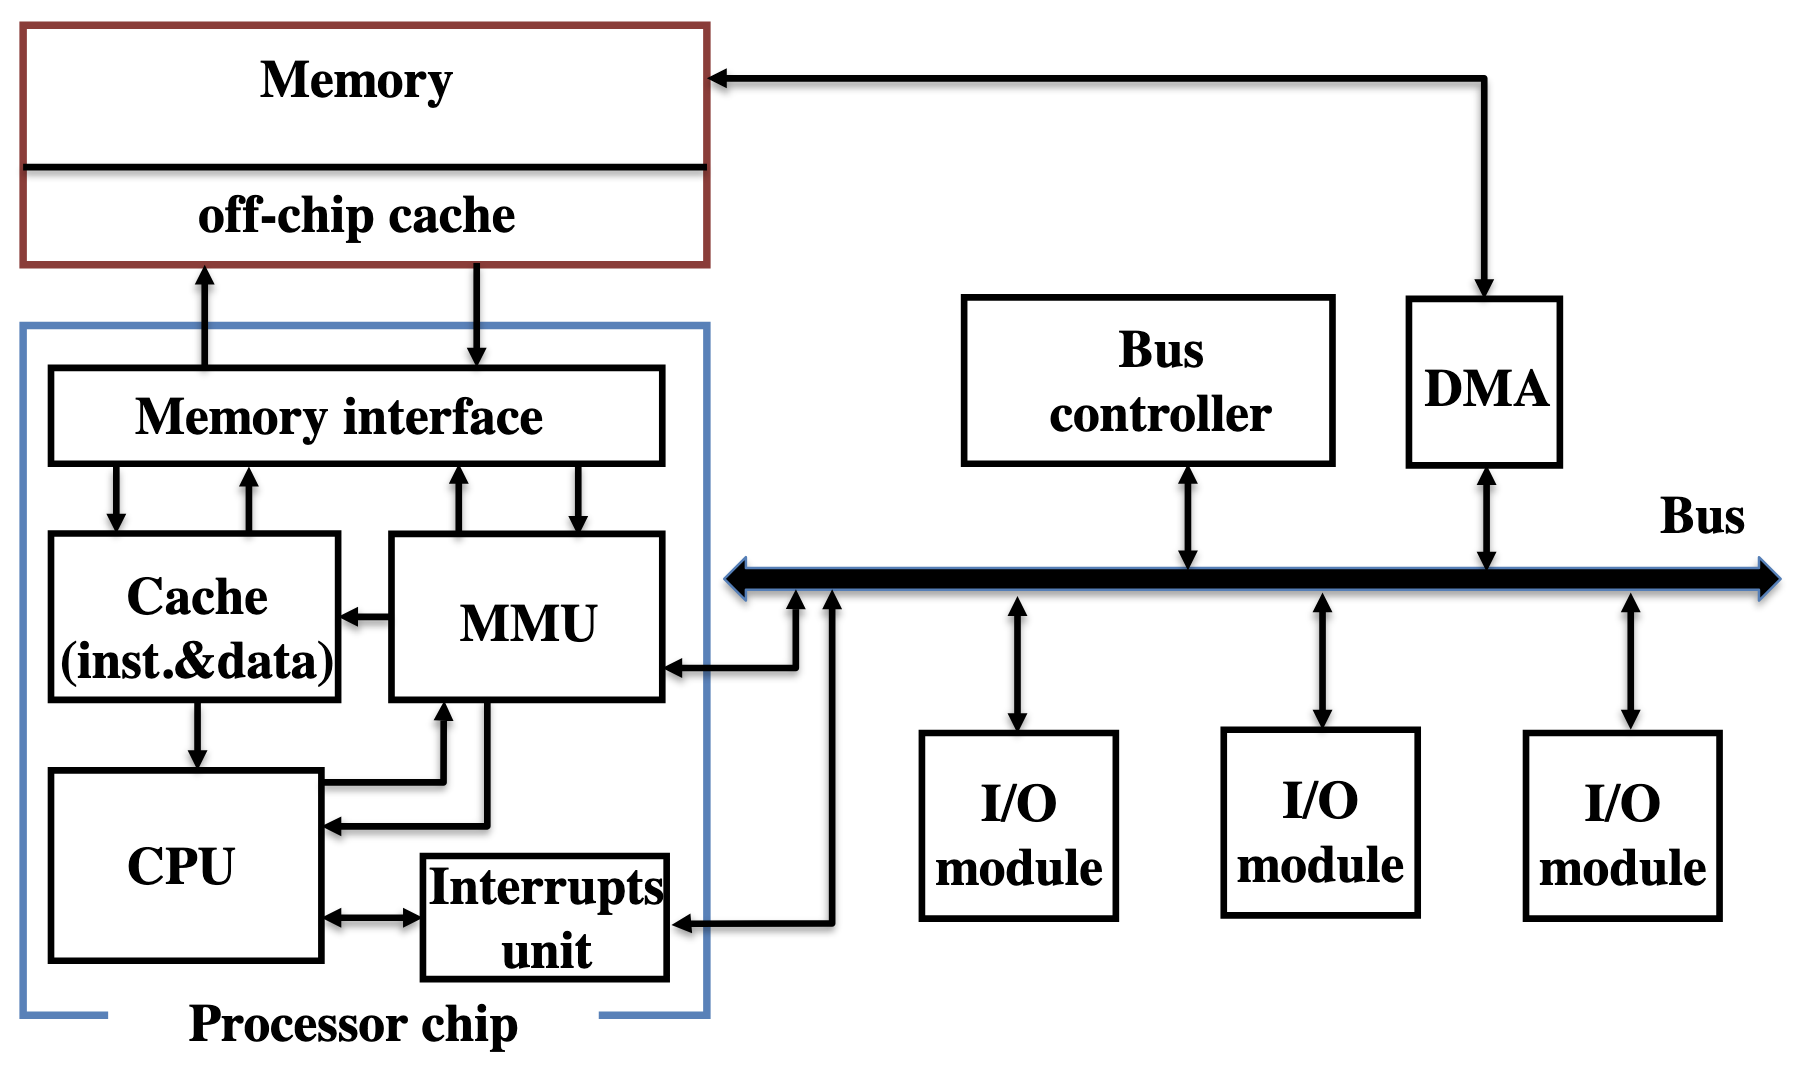
\includegraphics[width=6.5cm]{images/cache-based-architecture.png}
        \caption{}
    \end{subfigure}
\end{figure}
    

\subsection{Utilizzo della cache}
L'organizzazione della cache avviene non a blocchi ma a line, ogni linea contiene blocchi di memoria (8-16 memory words). la prima volta che il processore richiede la memory ad una cache miss succede che il blocco contenente la parola si trasferisce dentro la cache. \\
La richiesta successiva può essere di due tipologie:
\begin{itemize}
    \item \textbf{Cache hit}: se il dato è presente nel blocco.
    \item \textbf{Cache miss}: se il dato non è presente dentro il blocco. In questo caso il blocco che contiene il dato viene trasferito dentro la cache line.
\end{itemize}

Vediamo ora l'effetto della cache sul AMAT. Innanzitutto l'utilizzo di grandi cache nella gerarchia delle memorie aiuta a ridurre il bottleneck di von Neumann. 
\begin{example}
Vediamo un esempio quantitativo stabilendo dei valori:\\
$t_M = 50ns$ (main memory service time), $t_{L1} = 1ns$ (L1 hit time, cache hit service time). \\\\
Abbiamo un Miss rate ($MR_{L1}$) è del $5\%$, senza cache AMAT = 50ms mentre con L1 cache $AMAT = t_{L1} + MR_{L1} * t_M = 1 + 0.05 * 50 = 3.5ns$
\end{example}

\subsection{Cache performance}
\(CPU_{time} = ClockCycles * ClockCycleTime = IC * CPi * ClockCyleTime\) in qeusta formula abbiamo:
\begin{itemize}
    \item IC che è il numero di istruzioni che vengono effettivamente eseguite.
    \item CPI definito come \(\frac{clockcycles}{IC}\)
\end{itemize}

Bisogna sempre tenere conto di quando non è presente in cache. Quindi il calcolo del CPI deve tenere in conisderazione questo fattore, e per farlo si usa il seguente calcolo
\[CPI_{staff} = \frac{Memory Instructions}{Program Instructions} * MIss rate * Miss penality\]
\[CPi = (CPI_{Perfect} + CPI_{Stall})\]

\begin{example}
    Assumiamo che abbiamo un miss rate del \(2\%\) per la cache delle istruzioni mentre un \(4\%\) per la cache dei dati, ed una miss penality di 100 cicli per ogni mancanza, una frequenza Inoltre
    di \(36\%\) per le ldr, e le str. Se la CPI è 2 senza memory stalls, dobbiamo determinare quanto va più veloce un processore con una cache perfetta rispetto ad una cache reale (che ha le caratteristiche elencate sopra).\\

    \[CPI_{stall-instr} = 1 * 0.02 * 100 = 2 cycles\]
    \[CPI_{Stall-data} = 0.36 * 0.4 * 100 = 1.44 cycles\]
    \[CPi_{stall} = 2 + 1.44 = 3.44\]
    spendiamo quindi in media 3.44, e quindi in totale il nostro processore CPI = 2 + 3.44 = 5.44.

    \[\frac{CPU_{\text{time with stalls}}}{CPU_{time Perfect}} = \frac{IC * (CPI_{perfect} + CPI_{stall}) * Clockcycletime}{IC * CPI_{perfect} * ClockCycleTime} =  \frac{5.44}{2}\]
\end{example}

Tenendo quindi conto di questi aspetti negativi, possiamo andare ad agire su uno o più di questi fattori, andando a renderli il più bassi possibili.
\(AMAT = hit-time + miss-rate * miss-penalty\). Quindi possiamo:
\begin{itemize}
    \item Ridurre il miss rate
    \item Ridurre la miss penality
    \item Redurre l'hit time
\end{itemize}

\subsection{Design cache system}
Una delle prime domande che dobbiamo porci è come i dati sono organizzati.\\
Data una cache di una certa capacità C è organizzata come S sets in cui ciascuno contiene B block (o linee). b è il nnumero di parole per blocco.
Da qui possiamo distingure vari metodi di organizzaziazione:
\begin{enumerate}
    \item Direct mapped
    \item N-way set associatice, in cui N definisce il numero di blocchi conetnuti in un set quindi S=B/N
    \item Fully associative, in cui in questo caso nell'insieme c'è uno unico blocco contenente tutta la cache.
\end{enumerate}
Da ora andremo a considerare un sistema a 32-bit di indirizzi e 32-bit di parole quindi la memoria ha \(2^{30}\) parole.
Andimo ora a visualizzare la cache come una lista di indirizzi che parte da 0 ed arriva a quello finale. Avremo sempre i primi due bit a 0 per indicizare il bite.
La funzione di mapping diretta della cache è una funzione rigida.\\

\begin{wrapfigure}{r}{6.5cm}
    \centering
    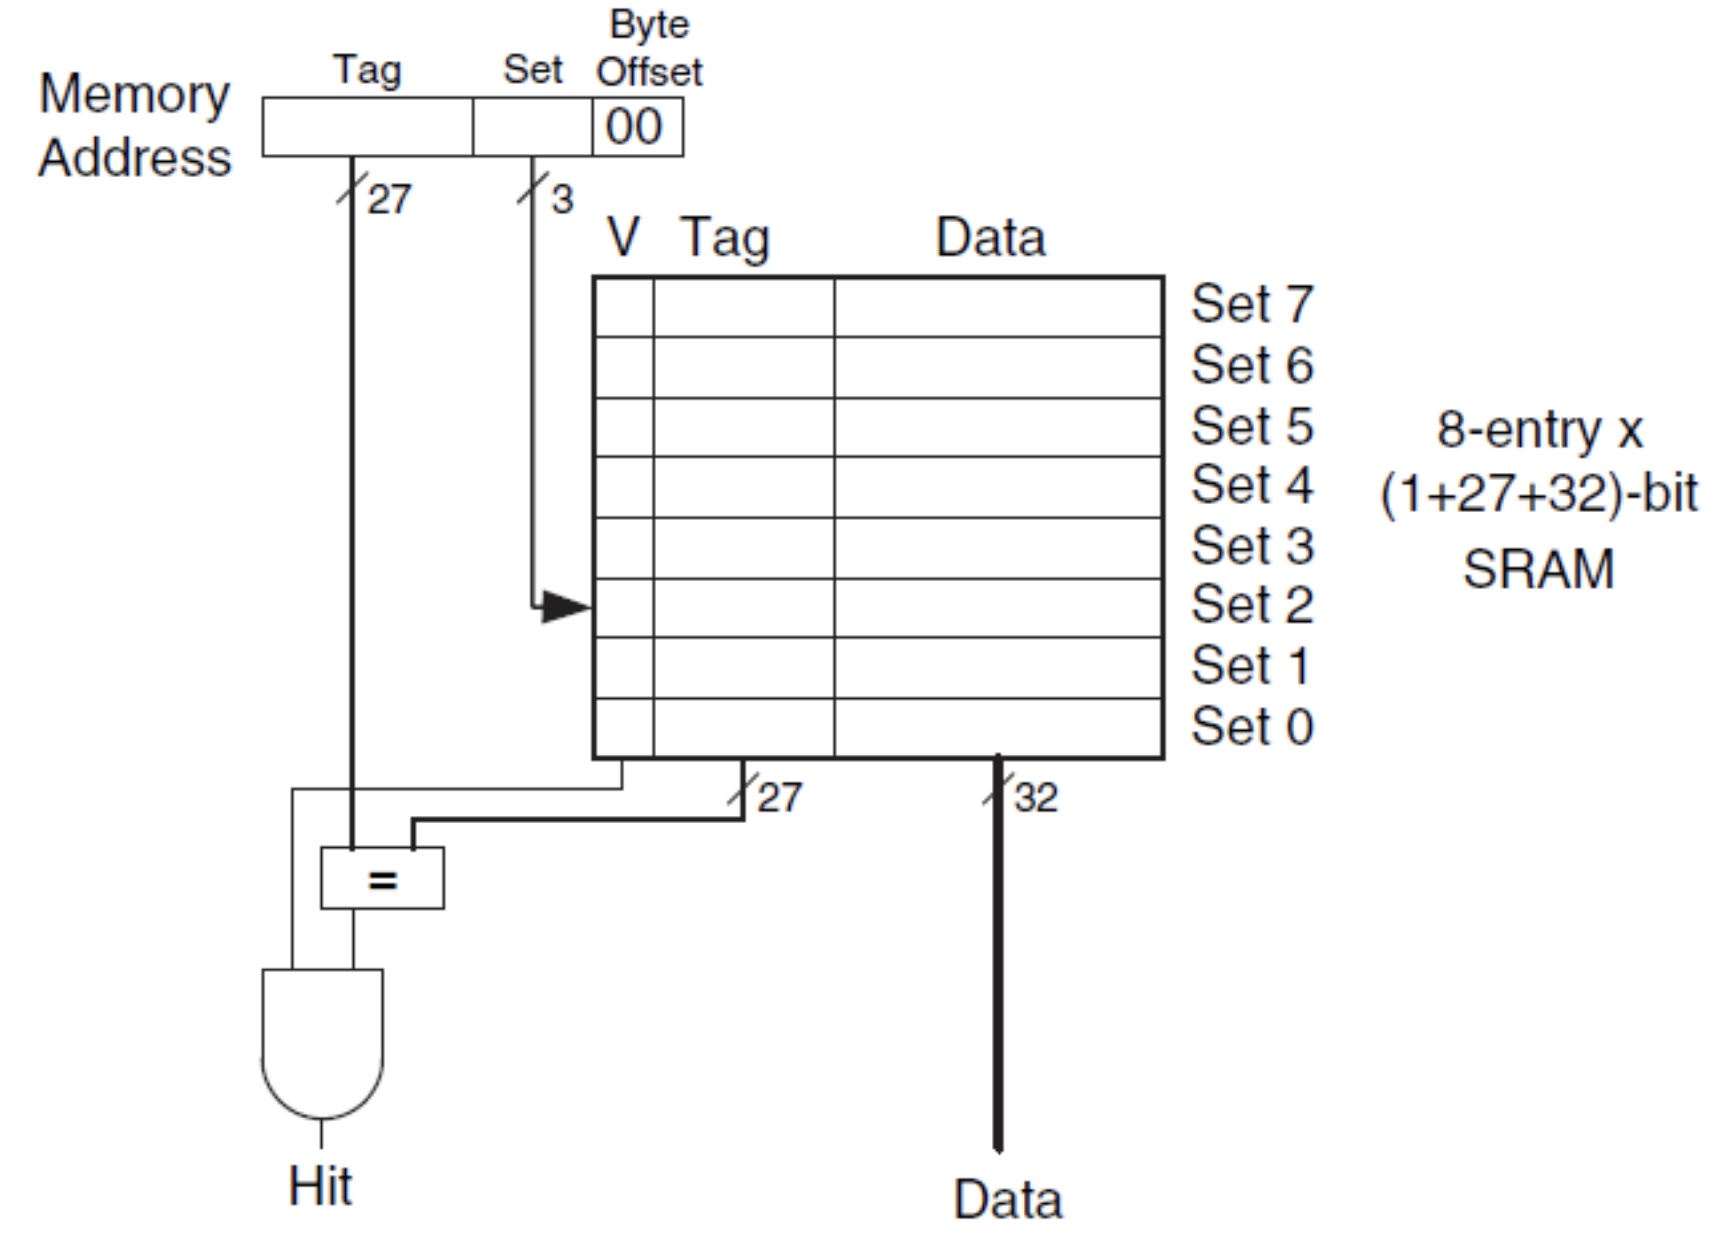
\includegraphics[width=6cm]{images/direct-mapped.png}
    \caption{Direcet mapped}
\end{wrapfigure}
%Riguarda le slide per l'esempio

Per capire dov mettere l'indice della tabella, cioè l'indice di blocco, e per capire se la parola che stiamo inserendo è quella giusta si va a prendere l'indirizzo e si va a
ragruppare.

%iinserisci immagine

Vediamo un caso realistico dove \(b > 1\), prndiamo C = 8 e b = 4, Abbiamo quindi B = C/b = 2 quindi S = 2, dobbiamo quind andare af "affettare l'indirizzo" nel seguente modo:
%inserisci immagine 

Vediamo un ultimo esempio. Questa è un cache  con una capacità C = 16k, S = B = 256, e b = 16. Avendo 16 parole dobbiamo prendere. V è il bit di validità, e ci dice se le parole seguenti
possono essere considerati valide o meno, perchè ci sono casi in cui vogliamo rendere invalido il blocco. I primi due byte di offset, in una parola di 32 bit abbiamo 4 byte 
%inserisci immagine + riguarda bene le slide

\begin{example}
    Supponiamo di avere indirizzi a 32 bit, una cache ad accesso diretto con S = B = 128 ed ognuna continen b = 8. Dobbiamo trovare la struttura con cui organizare gli indirizzi.\\
    Ci servono inanzitutto 2 bit per l'offset, poi ci servno \(log_2 8\) = 3 bits, dobiamo capire quanti bit ci servono per l'indice, che si calcolano con \(\log_2 129 = 7 bits\), la parte rimanete
    di bits sono per TAG ed è di 20 bits.
\end{example}

\begin{example}
    Supponiamo sempre di avere indirizzi a 32 bit, una cache ad accesso diretto con S = B = 128 ed ognuna continen b = 8. Dobbiamo caloclare la linea di cache e l'offset all'interno della linea
    di cache che conterra l'indirizzo 0xFFAC. 0xFFAC = 0...01111 1110 1010 1100 dove si può ragruppare in 3 parti fatte nel seguente modo (TAG, IDX, OFF) = (0...01111, 1110101, 01100). \\
    Quindi la liena di cache ha indice 117 quindi la 118th entry. L'offst nell blocco di cache è 3 quindi la 4th parola di memoria.
\end{example}

\begin{example}
    Consideriamo il seguente codice in C: for(i=0; i<16, i++) C[i] = A[i] + B[i]. Ed andiamo a considerare solamente le operazioni di ldr.\\
    Poi prendiamo un processore con 2Ghz con un mapping diretto L1 ai dati dalla cache con C = 128, b=8, \(t_m = 100\) cicli è \(t_{L1} = 4\) cicli. 'A' inizia all'indirizzo 0x00000000, 
    'B' inizia all'indirizzo 0x00000040 e 'C' inizia all'inidirizzo 0x00000080. %Il resto copialo dalle slide
\end{example}
\hspace{-15pt}Quindi per risasumere possiamo dire che i pro sono:
\begin{itemize}
    \item La realizzazione è semplice
    \item E' molto veloce in caso di hits
\end{itemize}
Mentre nel caso dei contro abbiamo:
\begin{itemize}
    \item La funzione di mapping a posizione fisse può generare potenzialmente molti conflitti.
    \item La troppa rigidità potrebbe avere un grosso impatto sul numero dei conflitti nella casch, essi dipendono dal posizionamento della memoria e dall'utilizzo delle strutture dati.
\end{itemize}

\begin{figure}[h!]
    \centering
    \begin{subfigure}{.45\textwidth}
        \centering
        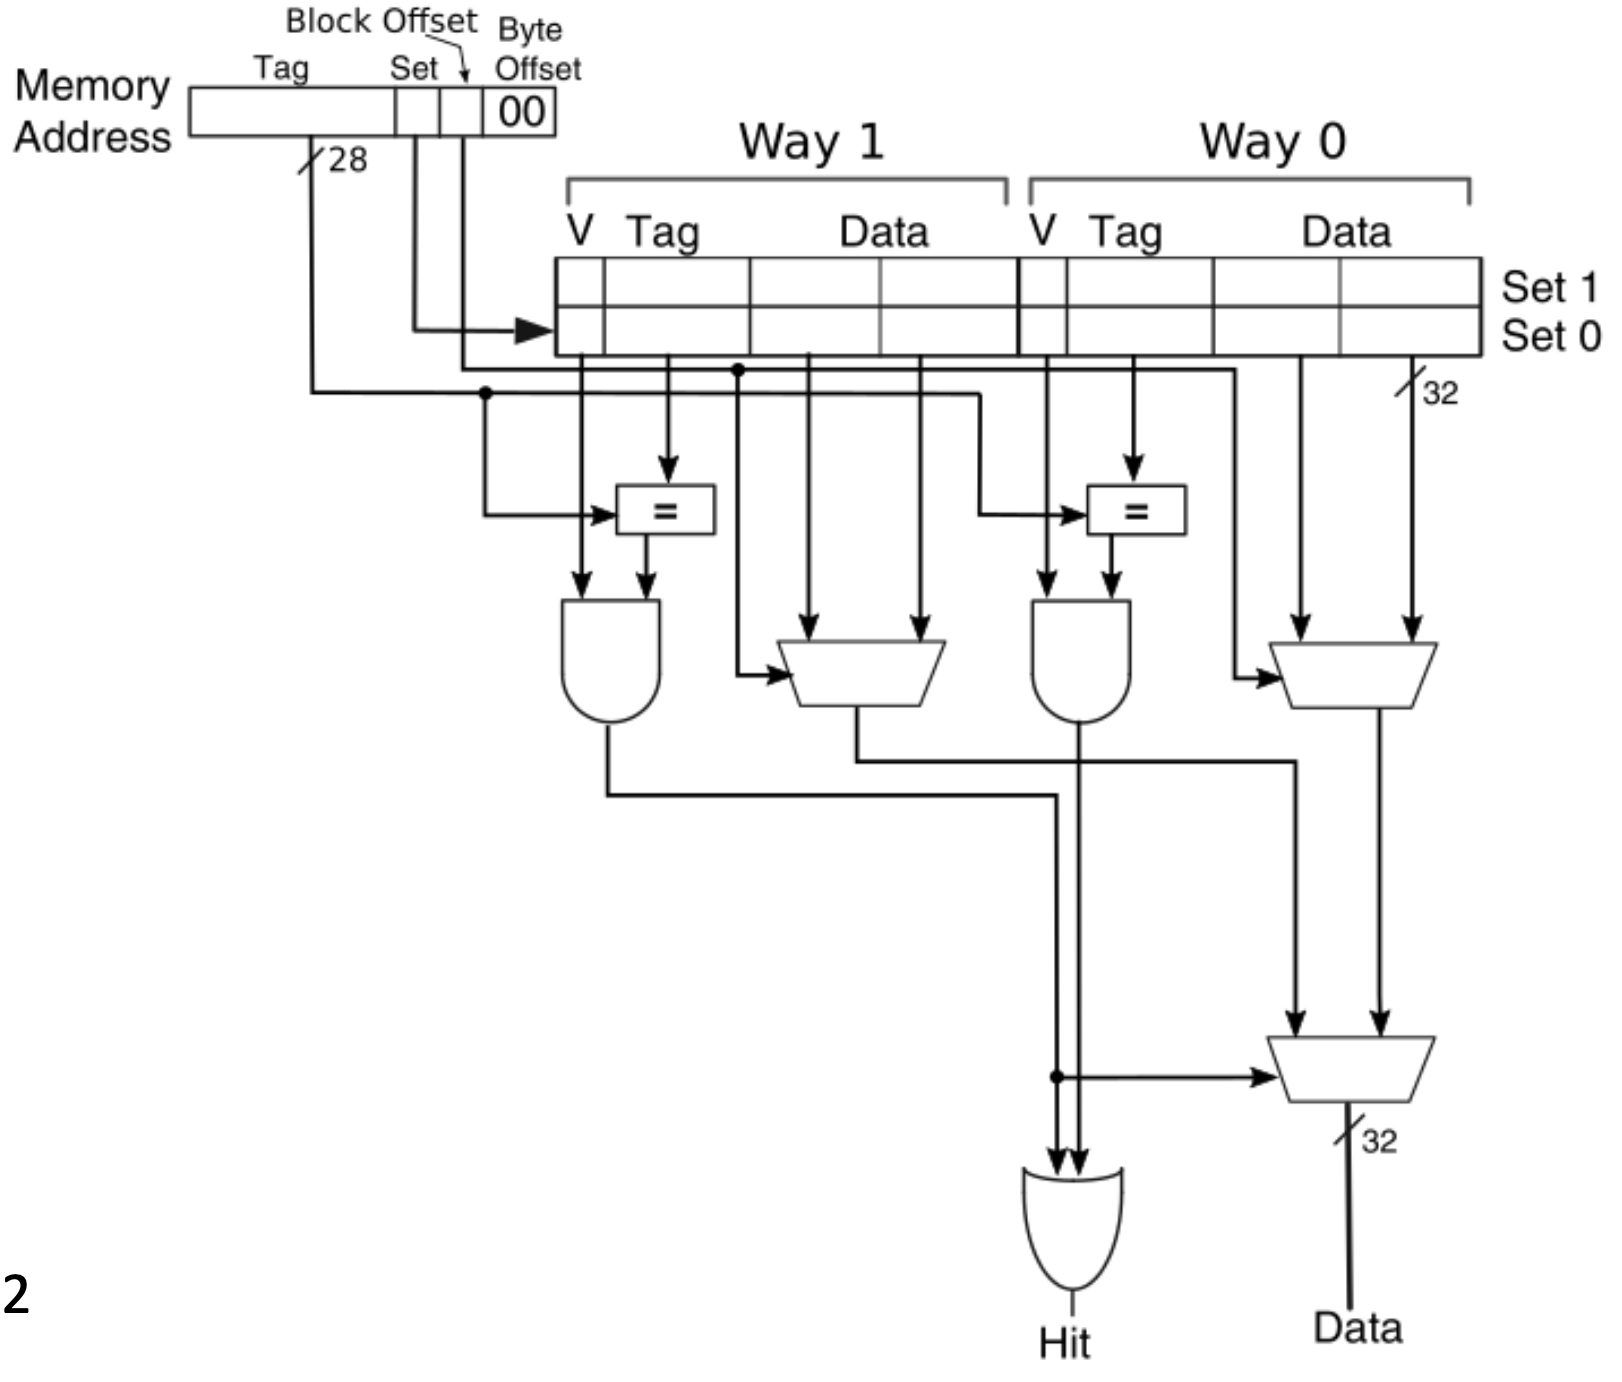
\includegraphics[width=4.7cm]{images/fully-associative.png}
        \caption{Fully associative}
    \end{subfigure}
    \begin{subfigure}{.45\textwidth}
        \centering
        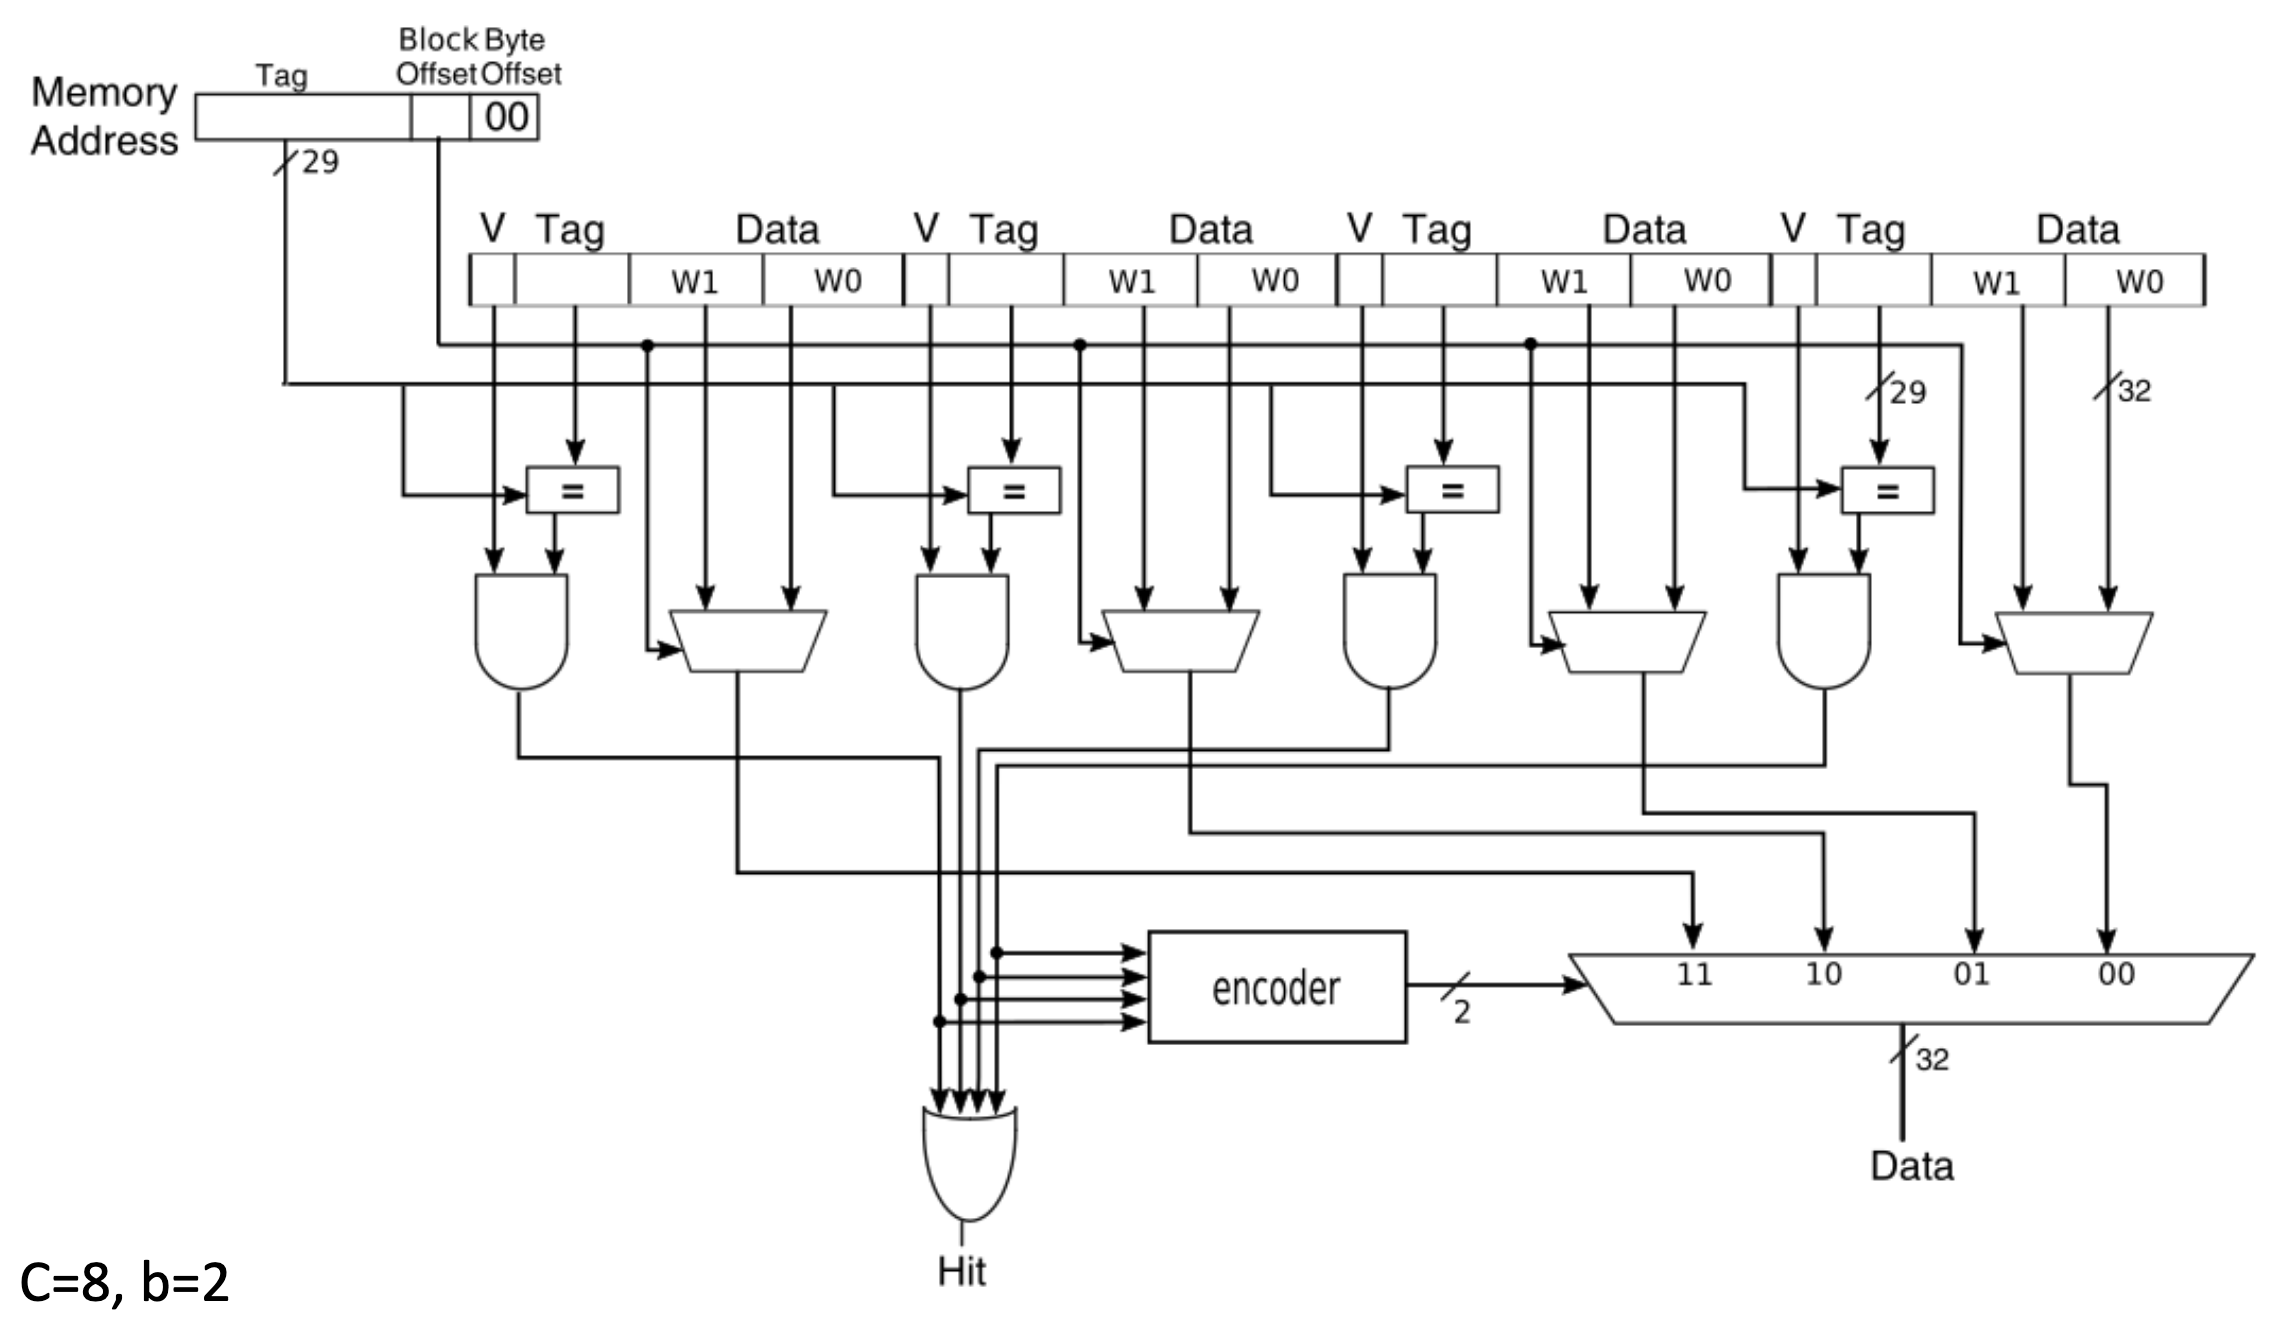
\includegraphics[width=4.7cm]{images/n-way-associative.png}
        \caption{N-way associative}
    \end{subfigure}
\end{figure}

\subsection{Cache associativa}
La cahce ad accesso diretto ha una funzione di mapping fissa ed un dato indirizzo può andare solo ad una linea di cache. Mentre una cache ad accesso indiretto possono essserci più indirizzi sulla stessa
linea di cache.
Che si divide a sua olta in cache Fully associative e N-way set-associative cache.


\subsection{Cache miss}
Le tipologie di cache miss sono le seguenti:
\begin{itemize}
    \item \textbf{Compulsory miss} questo tipologia di cache misses viene causato dal primo acceso al blocco che non è mai stato in cache.
    \item \textbf{Capacity miss} causato dalla cache che non coneinte tutti i bocchi necessari.
    \item \textbf{Conflict miss} solo per la mappatura diretta per i set associativi
\end{itemize}
A questo punto, visti i vari strumenti della cache e le tipologie di miss possnaimo andare  avedere come ridurre i cache miss tramite l'utilizzo di alcune tecniche:
\begin{itemize}
    \item \textbf{Aumentare la dimensione dei blocchi}. Andando così ad unmentare la località spaziale ma umentando anche la miss penalty.
    \item \textbf{Aumenteare l'associativià}. Meno conflitti ma un maggiore tempo di hit.
    \item \textbf{Aumentare dim. dei case}. Porta a meno capacity miss e conflitti ma aumenta l'hit time.
    \item \textbf{Usare algoritmi di cache-oblivius}.
\end{itemize}
In caso comunque avvengano dobbiamo andarli a gestire. Un errore nella cache blocca l'intero processore, congelando 
il contenuto di tutti i registri durante l'attesa della memoria: in effetti, un processore più avanzato consente l'esecuzione fuori ordine di altre istruzioni durante l'attesa della memoria.
Gli steps che vengono eseguiti per la gestione di un cache miss (\textbf{fautl management}):
\begin{enumerate}
    \item Indica al livello di memoria successivo di leggere il valore mancante.
    \item Attendi che la memoria risponda (questo può richiedere più cicli).
    \item Aggiorna la riga della cache corrispondente con i dati ricevuti.
    \item Riavvia l'esecuzione dell'istruzione (ora è un hit della cache).
\end{enumerate}


\subsection{Gestione delle scritture}
Dobbiamo definire quelle che sono le \textbf{write hits}, se l'istruzione di stroe scribe il dato soltanto dentro la cache, dopo la cache
è la memoria potrebbeero avere differenti valori (quindi abbiamo un inconsistenza).\\
Abbiamo poi \textbf{write miss}. 
\begin{itemize}
    \item Chiediamoci se possiamo recuperare il blocco dalla memoria alla cache e poi andiamo a sovrascivere la parola mancante?
    La risposta è si e questa policy si chiama \textbf{write-allocate}.
    Il blocco viene caricato nella cache seguito da un hit di scrittura (utilizzato principalmente nella politica Write-Back).
    \item Poi chiediamoci anche se dovremmo scrivere la parola direttamente al livello di memoria successivo? 
    Questa politica è chiamata \textbf{no-write-allocate}, il blocco non viene caricato nella cache (utilizzato principalmente nella politica Write-Through)
\end{itemize}

\subsubsection{Write-Through}
Gli hit di scrittura aggiornano sempre sia la cache che il successivo livello di memoria.
\begin{itemize}
    \item \textbf{Pro}: Soluzione semplice, facile da implementare. I dati sono sempre coerenti tra i due livelli di memoria.
    \item \textbf{Contro}: La velocità di scrittura dipende dalla velocità di scrittura del livello di memoria inferiore. Maggiore traffico di memoria, per ogni singola scrittura potrebbero esserci più scritture in ogni livello di memoria.
\end{itemize}

\subsubsection{Write-Back}
I colpi di scrittura aggiornano solo la cache, quindi il blocco modificato viene scritto nel livello di memoria inferiore quando viene sostituito. 
\begin{itemize}
    \item \textbf{Pro}: la velocità delle scritture è quella della cache: minore traffico di memoria rispetto a Write-Through, le successive scritture sullo stesso blocco di cache non producono traffico con il livello di memoria inferiore più costoso.
    \item \textbf{Contro}: 
    Abbiamo bisogno di tenere traccia dei blocchi modificati (bit sporchi). Più complesso da implementare rispetto al Write-Through. La sostituzione della riga della cache è più costosa.
\end{itemize}
Il write-back può migliorare le prestazioni specialmente quando la CPU genera istruzioni di memorizzazione più velocemente di quanto la memoria principale può gestire, tuttavia, il costo delle scritture nella cache è maggiore se si verifica un errore di scrittura, dobbiamo prima riscrivere il blocco in memoria (se il dirty bit è 1). 
Ciò richiede almeno due cicli anche per un hit di scrittura: un ciclo per verificare un hit seguito da un ciclo per eseguire effettivamente la scrittura. In alternativa, possiamo usare un buffer di scrittura per trattenere temporaneamente i dati da scrivere mentre il blocco della cache è controllato per un colpo. 
Il processore esegue la ricerca nella cache e inserisce i dati nel buffer di scrittura durante il normale ciclo di accesso alla cache. Supponendo un riscontro nella cache, i nuovi dati vengono scritti dal buffer di scrittura nella cache al successivo ciclo di accesso alla cache inutilizzato (pipelining degli accessi).

\subsubsection{Ottimizzare le scritture}
Poiché la scrittura nella memoria off-chip è costosa, gli archivi di memoria sono bufferizzati, un \textbf{buffer di scrittura} viene utilizzato per conservare i dati in attesa di essere scritti nella memoria.
L'esecuzione continua immediatamente dopo la scrittura dei dati nella cache e nel buffer di scrittura, la memoria memorizza nella memoria principale viene eseguita in parallelo con il calcolo della CPU, 
la CPU va in stallo solo se il buffer di scrittura è pieno, quindi la larghezza di banda richiesta dalla memoria principale è un fattore critico, in particolare per il modello di cache Writhe-Through!

\subsection{Cache replacement}
In una direct mapped cache, il blocco richiesto può andare esattamente in una posizione, quindi non abbiamo scelta: 
se il blocco da sostituire è stato modificato e la politica di scrittura è Write-Back, dobbiamo aggiornare la memoria di livello inferiore. 
Cache associativa, possiamo scegliere dove posizionare il blocco richiesto: 
\begin{itemize}
    \item Fully associative cache, tutti i blocchi sono candidati per la sostituzione.
    \item N-way set-associative cache, dobbiamo scegliere tra gli Nblocchi nel set selezionato.
\end{itemize}

\subsubsection{Cache replacement policy}
Per decidere quali blocchi andare a rimpiazzare si possono applicare delle policy di rimpiazzamento, alcune di queste sono:
\begin{itemize}
    \item Lo schema più utilizzato è \textbf{Least Recent Used (LRU)}. Considera la località temporale, il blocco sostituito è quello che è rimasto inutilizzato per il tempo più lungo. 
    Per una cache set-associativa a 2 vie, può essere implementato con 1 bit (usare bit --U), per un 4 vie è ancora fattibile con 2 bit, per più di 4 vie diventa abbastanza complicato (pseudo-LRU).
    \item Per le cache altamente associative, una politica \textbf{Random} offre all'incirca le stesse prestazioni di LRU.
\end{itemize}

\begin{example}
    Considera una piccola cache con 4 blocchi, b=1. Trova il numero di errori per una cache a mappatura diretta per la seguente sequenza ordinata di indirizzi di blocco 0, 8, 0, 6, 8.
\end{example}

\subsection{Designing the Memory System}
La penalità di errore può essere ridotta aumentando la larghezza di banda del bus tra DRAM e cache. Ci sono tre possibili organizzazioni:
\begin{itemize}
    \item \textbf{Semplice}: una parola alla volta viene letta dalla memoria.
    \item \textbf{Ampia memoria}: N parole alla volta vengono lette dalla memoria.
    \item \textbf{Interleaved}: K banchi di memoria indipendenti in grado di servire K richieste contemporaneamente.
\end{itemize}
Consideriamo il tempo di trasferimento del blocco della cache per l'organizzazione della memoria Simplevs Interleaved.

\subsection{Problemi cache}
La memorizzazione nella cache è essenziale per ridurre il collo di bottiglia di von Neuman e ottenere prestazioni ragionevoli sui sistemi moderni•Tuttavia, la memorizzazione nella cache introduce alcuni problemi nei sistemi multiprocessore/multicore. 
Problema di coerenza della cache, salsa condivisione degrado delle prestazioni nei multiprocessori coerenti con la cache, due variabili non correlate sono collocate nello stesso blocco della cache e accesso in modalità lettura/scrittura da thread diversi!

\subsubsection{Problemi di corerenza}
Supponiamo un'architettura SMP: SMP: Symmetric Multiprocessors, caching di dati privati e condivisi, i dati core privati vengono memorizzati nella cache in L1, riducendo così l'AMAT e le comunicazioni di memoria off-chip. 
Quando i dati condivisi vengono memorizzati nella cache, i valori condivisi può essere replicato in più core cache private. Questo riduce anche la contesa di memoria! Cosa succede se i dati condivisi vengono scritti? 
La memorizzazione nella cache dei dati condivisi introduce un nuovo problema: \textbf{la coerenza della cache}.

\subsubsection{Write invalidate protocol}
Il protocollo di invalidazione della scrittura invalida le copie dei dati presenti in altre cache durante un'operazione di scrittura. 
Una semplice implementazione utilizza un protocollo bus di snooping per garantire che il processore acquisisca l'accesso esclusivo a un blocco di cache prima che scriva in esso.
